\chapter{Аналитический раздел}

\section{Подходы к представлению реляционных БД}
\vspace{-0.5cm}
Подходы к организации хранения данных в БД можно представить при помощи разных моделей \cite{dbms_approaches}. Приведем некоторые из них по определению Р. Рейтера \cite{approach_reiter}:
\begin{itemize}
	\vspace{-0.3cm}
	\item[$\circ$] теоретико-модельный;
	\vspace{-0.4cm}
	\item[$\circ$] теоретико-доказательный.
\end{itemize}

Ключевые понятия, описывающие эти подходы, представлены в таблице \ref{table:dbms_approaches}.

\begin{table}[ht!]
	\centering
	\captionsetup{singlelinecheck = false, justification=raggedright}
	\caption{Подходы к организации хранения данных в БД}
	\label{table:dbms_approaches}
	\begin{tabular}{|c|c|}
		\hline
		\textbf{Теоретико-модельный} & \textbf{Теоретико-доказательный} \\ \hline
		интерпретация & гипотеза \\ \hline
		модель & доказательство теоремы \\ \hline
		реляционная структура & база знаний \\ \hline
	\end{tabular}
\end{table}

В теоретико-модельном подходе основным компонентом представления данных является \textit{таблица}. С математической точки зрения она представляет собой декартовое произведение $D_1,...D_n$ доменов. Другими словами, содержит множество кортежей вида $\langle x_1,...,x_i,...,x_n \rangle; i =\overline{1, n}$, включающее схему отношения.

Теоретико-доказательный подход основывается на исчислении предикатов первого порядка. Использование дизъюнктов Хорна позволяет описывать отношения в виде составного терма вида $f(t_1,...,t_n)$, где $t_1,...,t_n$ также являются термами, описанные с использованием доменов.

Р. Ковальски \cite{approach_kowalski} и Р. Рейтер \cite{approach_reiter} показали, что представление баз данных может быть рассмотрено как с теоретико-модельной, так и с доказательной точек зрения. Особенности, присущие каждому из перечисленных способов организации данных, представлены в таблице \ref{table:features_approaches}.

\begin{table}[ht!]
	\centering
	\captionsetup{singlelinecheck = false, justification=raggedright}
	\caption{Особенности представления модели в SQL и логических ЯП}
	\label{table:features_approaches}
	\begin{tabular}{|c|c|c|}
		\hline
		\textbf{Модель} & \textbf{SQL} & \textbf{Логические ЯП} \\ \hline
		База данных & Таблица & Набор термов \\ \hline
		Описание записи& Кортеж & Терм \\ \hline
	\end{tabular}
\end{table}

Каждое отношение характеризуется своим именем и списком именованных атрибутов. Такой упорядоченный набор значений является кортежем в реляционном случае. Для логического подхода такую основу составляет использование составного терма. Общий вид представлен в формуле \eqref{eq:general_view}.
\begin{equation}
	\label{eq:general_view}
	R(A_1, A_2,...,A_n),
\end{equation}
где $R$ -- имя отношения, а $A_i$ -- атрибуты; $i = \overline{1, n}$. Важным свойством для предикатов является то, что они не имеют атрибутов. Единственным способом, при котором можно указывать на домен, является позиция терма $A_i$.

Связь этих моделей представлена на рисунке \ref{image:predicates_general} \cite{logica}.
\begin{figure}[H]
	\centering{
		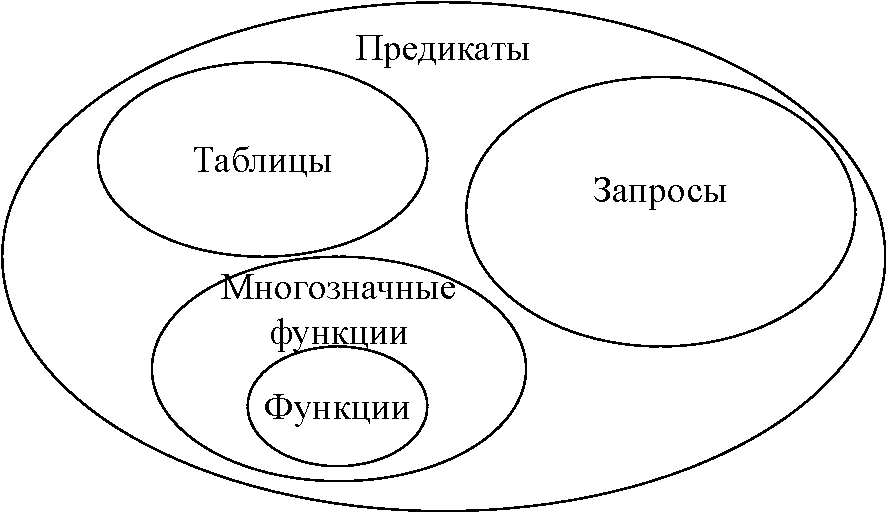
\includegraphics[scale=0.72]{./images/predicates_general.pdf}
		\caption{Связь моделей.}
		\label{image:predicates_general}
	}
\end{figure}

\section{Теория множеств и базы данных}
\vspace{-0.5cm}
Взаимосвязь данных в БД осуществляется при помощи описания множеств -- совокупности элементов, обладающих некоторым общим свойством. Используя данное понятие, можно построить более сложные и содержательные объекты. 

Известно, что алгебра есть множество вида $A = \langle H, S \rangle$, где H -- носитель (множество отношений), S -- сигнатура (множество операций над отношениями).
В реляционном случае над множествами R1 и R2 поддерживаются такие стандартные теоретико-множественные операции, как объединение ($R_1\cup R_2$), пересечение ($R_1\cap R_2$), разность ($R_1\setminus R_2$), декартово произведение ($R_1 \times R_2$). Логика первого порядка имеет свой набор операций: отрицание ($\neg$), конъюнкция ($\land$), дизъюнкция ($\lor$) и др, кванторы существования ($\exists$), общности ($\forall$) и т.д. Таким образом, логическая программа может быть использована для выражения практически любой операции реляционной алгебры.

\section{Обработка SQL-запроса}
\vspace{-0.5cm}
Подход к выполнению SQL-запроса в СУБД представлен на рисунке \ref{image:query_plan}.
\begin{figure}[H]
	\captionsetup{justification=centering}
	\centering{
		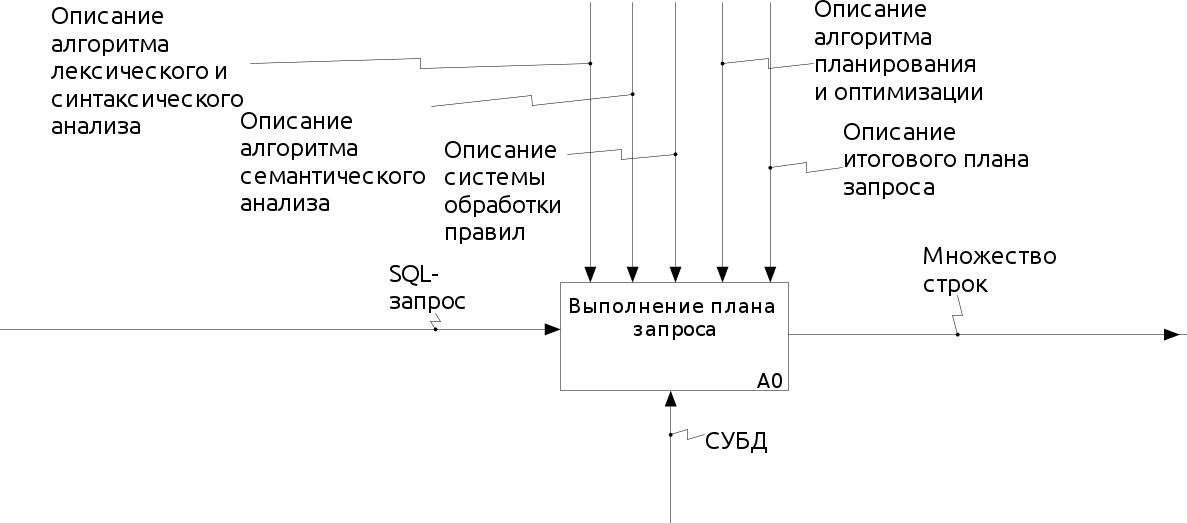
\includegraphics[scale=0.41]{./images/plan_sql.png}
		\caption{Выполнение SQL-запроса в СУБД.}
	    \label{image:query_plan}
    }
\end{figure}
Для выполнения запроса СУБД требуется в качестве входных данных составленный некоторый SQL-запрос. После пройденных этапов выполнения его обработки в результате будут получены строки, удовлетворяющие ему.
Алгоритмы лексического, синтаксического, семантического анализа, планирования и оптимизации, а также система обработки правил определяется конкретной СУБД.

\section{Структура плана запроса}
\vspace{-0.5cm}
Плана запроса можно представить в виде древовидной структуры, имеющей множество уровней. На нижнем находятся те узлы, на которых выполнялось сканирование таблицы для доступа к данным. При необходимости таких операций как объединение, сортировка, агрегатные вычисления и др. соответствующие узлы добавляются над узлами сканирования. Пример такого дерева с ограниченной грамматикой SQL (содержатся основные операторы SELECT, FROM, WHERE) представлен на рисунке \ref{image:parse_query_tree}.

\begin{figure}[H]
	\captionsetup{justification=centering}
	\centering{
		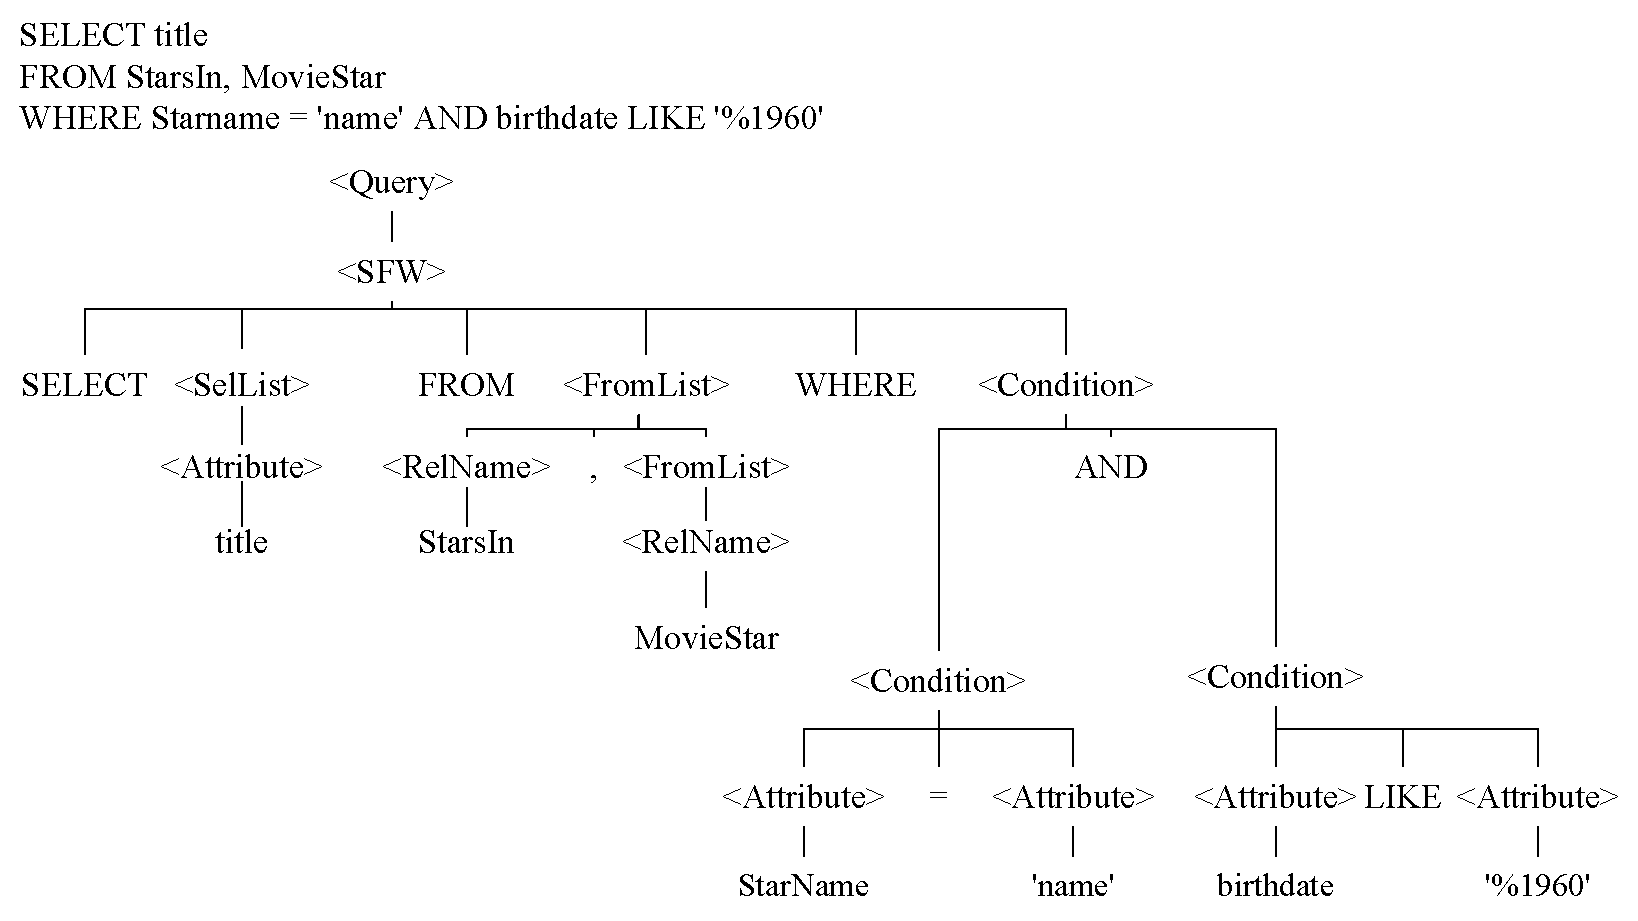
\includegraphics[width=\linewidth]{images/query_tree.pdf}
		\caption{Дерево плана запроса с ограниченной SQL-грамматикой.}
		\label{image:parse_query_tree}
	}
\end{figure}

\section{План выполнения запроса}
\vspace{-0.5cm}
План выполнения запроса действует как дерево инструкций, которым должен следовать механизм выполнения запроса для получения результатов. Он показывает, как будут сканироваться таблицы; если необходимо связывание нескольких таблиц, то какой алгоритм будет выбран для объединения считанных строк. Выполнение плана на верхнем уровне представлено на рисунке \ref{image:dfd_lvl0}.

\begin{figure}[H]
	\centering{
		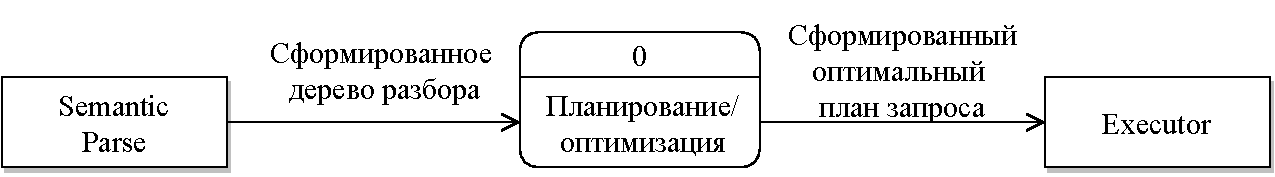
\includegraphics[scale=0.73]{./images/dfd_level_0.pdf}
		\caption{Выполнение запроса (верхний уровень).}
		\label{image:dfd_lvl0}
	}
\end{figure}

\section*{Вывод}
\vspace{-0.5cm}
В данном разделе были рассмотрены подходы к представлению реляционных баз данных, а также моделей в SQL и логичеcких языках программирования. Приведено применение теории множеств к базам данных: предикаты позволят лингвистически проще описать знания, а логика предикатов может выражать почти любые операции реляционной алгебры. Описаны обработка SQL-запроса, план запроса и его структура в ограниченной грамматике SQL. 